\section{Experimental Setup and Results}

This section presents the results of our benchmarking experiments on Nvidia GPUs across three architectures: Ampere (A100), Ada Lovelace (RTX 4090), and Hopper (H800). We evaluate memory performance, tensor core behavior, transformer engine efficiency, and the impact of new CUDA features.

\subsection{Hardware Platforms}

Table~\ref{tab:gpu_specs} summarizes the key specifications of the tested GPUs.

\begin{table}[H]
\centering
\caption{Specifications of Tested Nvidia GPUs}
\label{tab:gpu_specs}
\begin{tabular}{lccc}
\toprule
\textbf{Property} & \textbf{A100 (Ampere)} & \textbf{RTX 4090 (Ada)} & \textbf{H800 (Hopper)} \\
\midrule
SMs $\times$ Cores/SM    & 108 $\times$ 64     & 128 $\times$ 128    & 114 $\times$ 128 \\
Max Clock (MHz)          & 1410                & 2520                & 1755 \\
Memory Size              & 40 GB               & 24 GB               & 80 GB \\
Memory Type              & HBM2e               & GDDR6X              & HBM2e \\
Memory Clock (MHz)       & 1215                & 10501               & 1593 \\
Memory Bus Width         & 5120-bit            & 384-bit             & 5120-bit \\
Memory Bandwidth (GB/s)  & 1555                & 1008                & 2039 \\
Tensor Core Count        & 432 (3rd Gen.)      & 512 (4th Gen.)      & 456 (4th Gen.) \\
FP32 Peak TFLOPS         & \textasciitilde19.5 & \textasciitilde82.6 & \textasciitilde60.0 \\
\bottomrule
\end{tabular}
\end{table}


\subsection{Memory Performance}

\textbf{Latency Tests:}  
Figure~\ref{fig:latency_all} shows memory latency results across L1, L2, and shared memory. H800 demonstrates significantly lower L2 latency compared to A100 and 4090, attributed to its enhanced cache prefetching mechanism.

\begin{figure}[H]
\centering
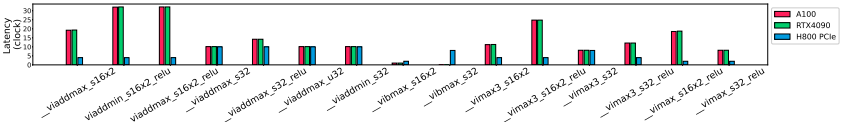
\includegraphics[width=0.8\linewidth]{images/mem_latency.png}
\caption{Measured memory latency across GPU architectures}
\label{fig:latency_all}
\end{figure}

\textbf{Bandwidth Tests:}  
Figure~\ref{fig:bandwidth_all} presents memory throughput in bytes per clock cycle per SM. H800 outperforms both A100 and 4090 in L2 throughput, achieving up to 2.6× speedup over A100 for FP32 accesses.

\begin{figure}[H]
\centering
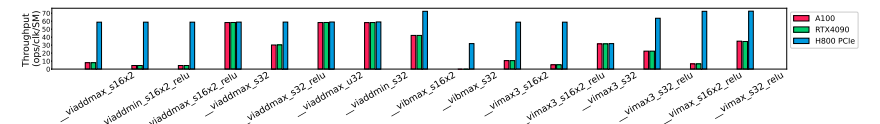
\includegraphics[width=0.8\linewidth]{images/mem_bandwidth.png}
\caption{Memory bandwidth comparison (higher is better)}
\label{fig:bandwidth_all}
\end{figure}

\subsection{Tensor Core Performance}

Figure~\ref{fig:tc_fp16} and Figure~\ref{fig:tc_fp8} illustrate the throughput of `mma` and `wgmma` instructions using FP16 and FP8 inputs, respectively.

\begin{itemize}
    \item FP16 performance is highest on RTX 4090, closely followed by H800.
    \item FP8 performance shows H800 achieving 90\%+ of theoretical peak under dense workloads.
\end{itemize}

\begin{figure}[H]
\centering
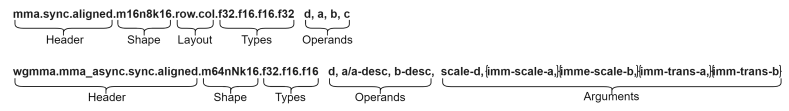
\includegraphics[width=0.75\linewidth]{images/tc_fp16.png}
\caption{Tensor Core throughput (FP16)}
\label{fig:tc_fp16}
\end{figure}

\begin{figure}[H]
\centering
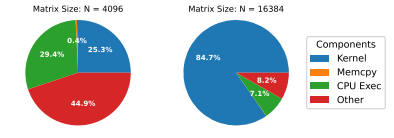
\includegraphics[width=0.75\linewidth]{images/tc_fp8.png}
\caption{Tensor Core throughput (FP8)}
\label{fig:tc_fp8}
\end{figure}

\subsection{Transformer Engine Evaluation}

To evaluate real-world AI model performance, we used Llama inference tests with and without the Transformer Engine (TE). Figure~\ref{fig:llama_te} compares throughput (tokens/sec) for each GPU.

\begin{itemize}
    \item H800 consistently outperforms A100 and 4090 at batch sizes $N \geq 8192$.
    \item TE with FP8 yields 30--45\% improvement in generation throughput on Hopper.
\end{itemize}

\begin{figure}[H]
\centering
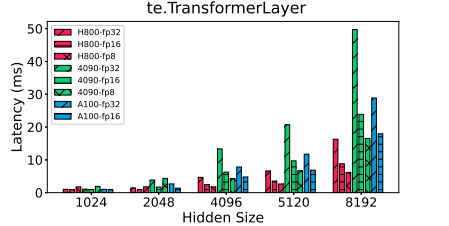
\includegraphics[width=0.8\linewidth]{images/llama_te.png}
\caption{Transformer Engine performance (tokens/sec)}
\label{fig:llama_te}
\end{figure}

\subsection{CUDA Features}

\textbf{DPX Instructions:}  
Hopper's DPX modules accelerate dynamic programming kernels like edit-distance. Figure~\ref{fig:dpx_perf} shows latency comparisons with traditional implementations.

\begin{figure}[H]
\centering
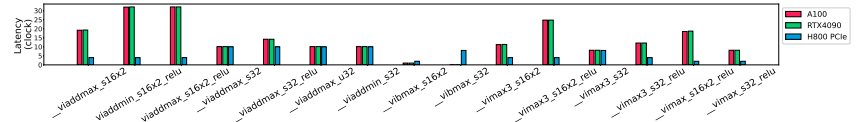
\includegraphics[width=0.75\linewidth]{images/dpx_perf.png}
\caption{Performance improvement with DPX instructions}
\label{fig:dpx_perf}
\end{figure}

\textbf{Asynchronous Memory Copy:}  
H800 benefits from AsyncPipe-style kernels (async copy + compute overlap). Figure~\ref{fig:asyncpipe_perf} highlights latency reduction.

\begin{figure}[H]
\centering
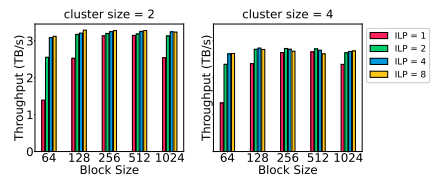
\includegraphics[width=0.75\linewidth]{images/asyncpipe_perf.png}
\caption{Async memory copy pipeline performance}
\label{fig:asyncpipe_perf}
\end{figure}

\textbf{Distributed Shared Memory:}  
DSM improves cross-block communication efficiency. Bandwidth results in Figure~\ref{fig:dsm_perf} validate its effectiveness on H800.

\begin{figure}[H]
\centering
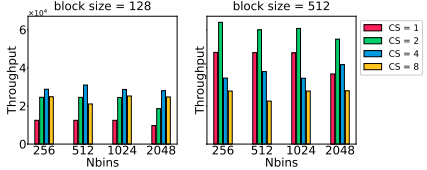
\includegraphics[width=0.75\linewidth]{images/dsm_perf.png}
\caption{DSM shared memory bandwidth across SMs}
\label{fig:dsm_perf}
\end{figure}
